%!TEX root = ../main.tex
%
% 波の性質
%


\section{気柱の固有振動と音速の測定}

\subsection{気柱の固有振動}

瓶の口に唇をあて、息を吹きかけると「ボー」といった一定の高さの音が発生することがあります。また、
笛やリコーダーといった管楽器では、指で抑える穴によって音程を変えることができます。
これは、管状のものの中にある空気({\bf 気柱})では音波と音波が重なり合い、定常波ができるからです。

管内の気柱が共鳴し定常波が発生する際の音波の振動数は、気柱の大きさや形状によって決まります。その時の振動数を
{\bf 固有振動数}と呼びます。

簡単のために、一定の半径を持った円筒状の管の気柱を考えることにすると、一方の端が開いていて他方の端が閉じている
管を{\bf 閉管}といい、両方の端が開いた管を{\bf 開管}といいます。今回の実験では、閉管を用い、開いた端からスピーカーを
使って音を入れます。

\subsection{閉管の場合}

\begin{wrapfigure}[16]{r}{7.5cm}
\vspace*{-0.8cm}
\begin{center}
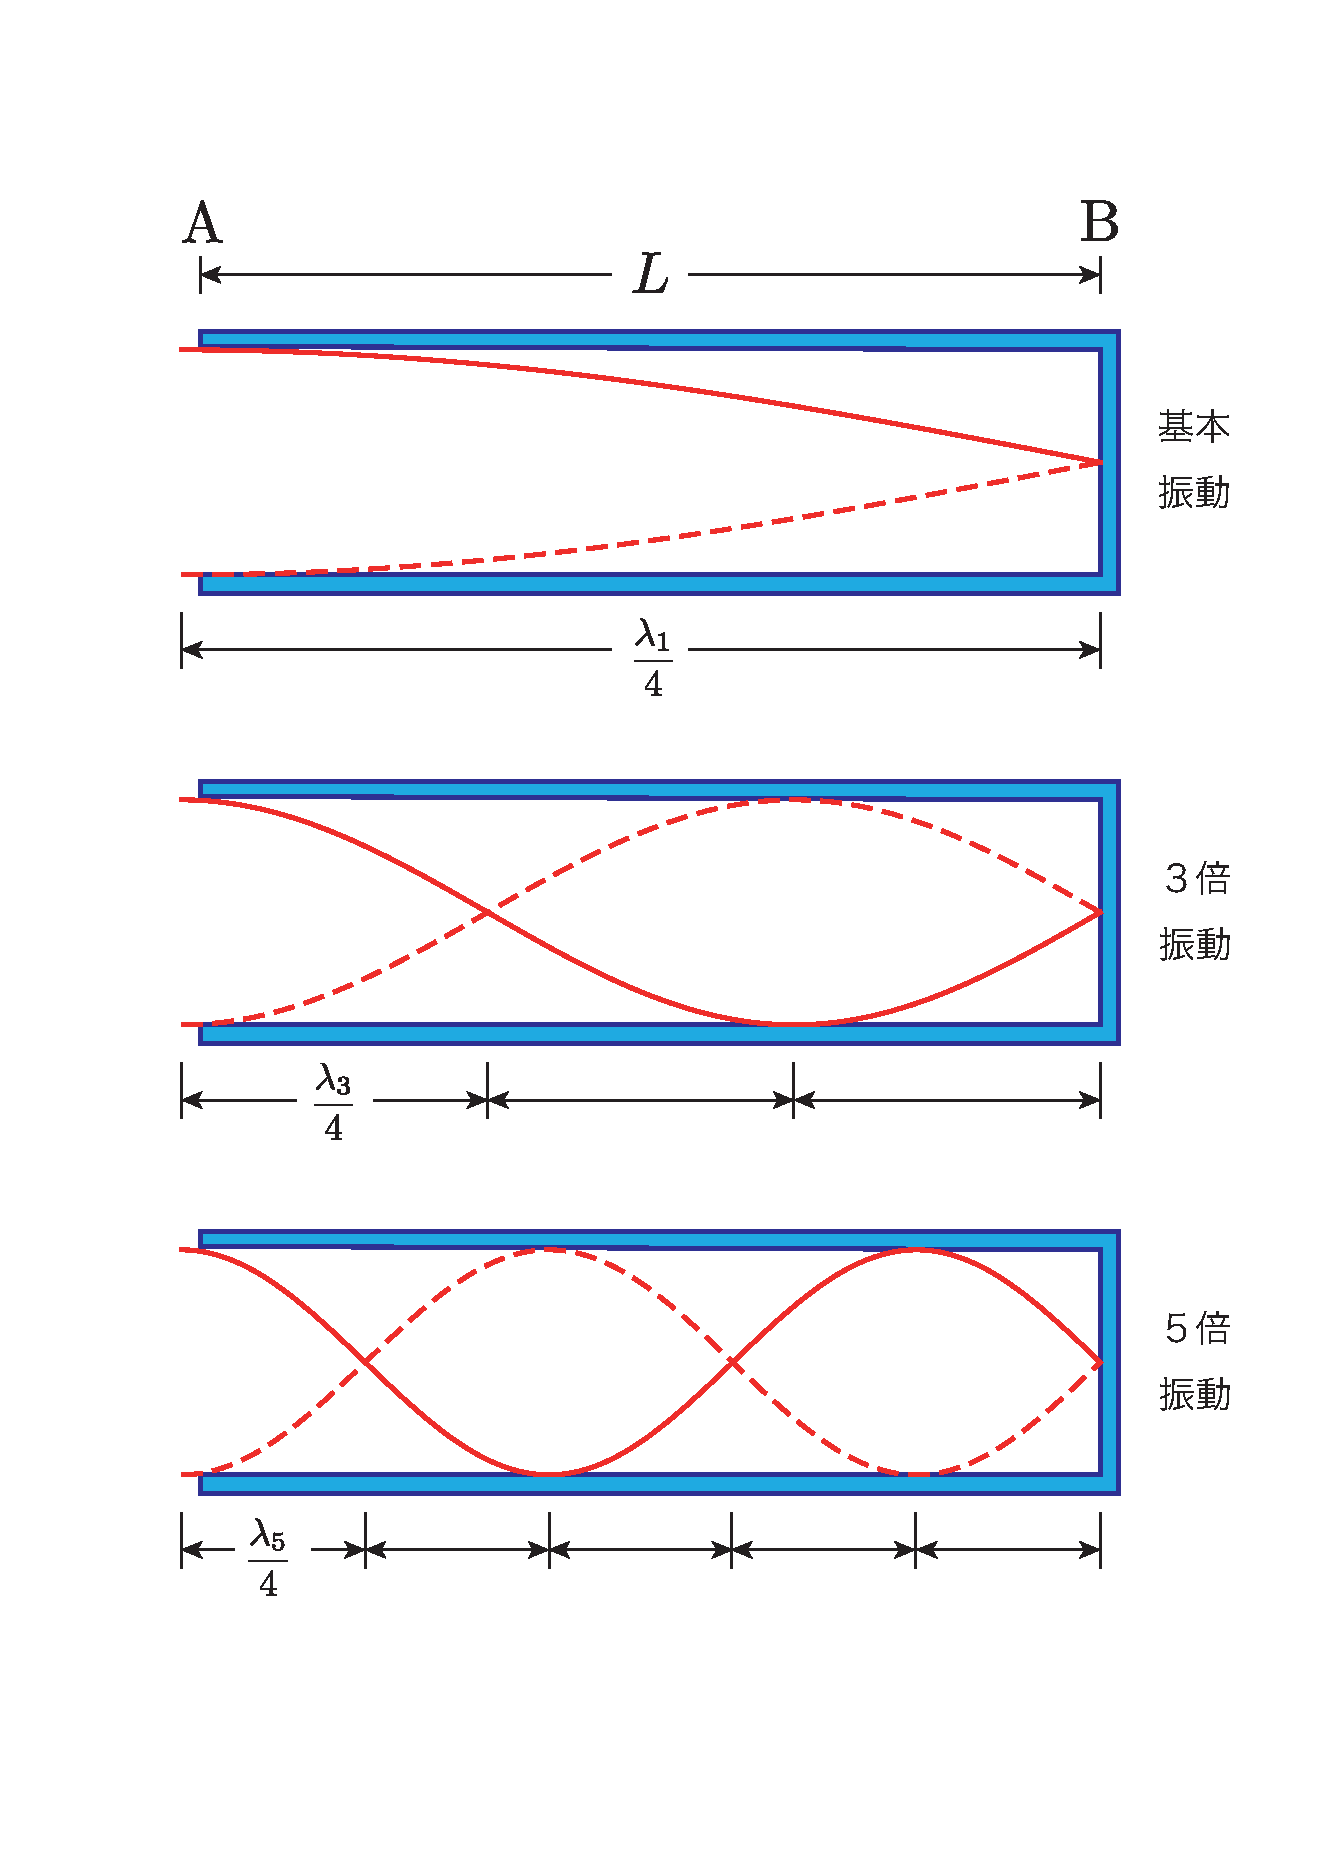
\includegraphics[scale=0.4]{18_Resonance/AirColumn.eps}\\
気柱(閉管)の固有振動\\
\end{center}
\end{wrapfigure}


スピーカーを使って閉管に入れた音の振動数を変化させると、いくつかの決まった振動数で音が強く響き({\bf 共鳴})、
気柱に定常波が発生します。スピーカーから出た音と閉管の閉じた端から反射した音が重なり合って定常波が発生するためには、
長さ$L$の気柱に、波長の$\frac{1}{4}$の長さがちょうど奇数個分入る必要があります(右図参照)。

音波が気柱に定常波を作るとき、開口端では空気が自由に振動できる自由端であるため、「腹」
となります。(空気が自由に移動できるということは、管の外の空気と同じとなるため、
腹の周りでは空気の密度変化が最も小さくなります。)
一方、閉口端では空気が振動できないため、その周りでは空気の密度変化が最も大きい「節」となります。

気柱が共鳴を起こしているとき、最も小さい振動数$\nu_1$では、開口端と閉口端だけで腹と節が生じます。このときの固有振動を
{\bf 基本振動}といいます。

振動数を大きくしていくと、基本振動数$\nu_1$ の3倍、5倍、7倍、$\cdots$となったときに
管の両端以外にも図のような腹と節が発生します。このときを、それぞれ、
3倍振動、5倍振動、7倍振動、$\cdots$と呼びます。

\subsection{空気中の音の速さ}

$n$倍振動($n=1,3,5,7,\cdots$)が発生したとき、節と節の間隔や腹と腹の間隔を測定すると、その間隔は音波の波長の
ちょうど半分になっているので、音波の波長を求めることができます。また、気柱の長さからでも波長を求めることが
できますが、開口端側の腹の位置は管の外側にややずれているため、注意(開口端補正)が必要です。
(振動数を固定し、異なる$n$倍振動が発生したときの管の長さを複数回測定することで開口端補正をすることができます。)

$n$倍振動時の気柱の固有振動数$\nu_n$と、そのときの波長$\lambda_n$がわかれば、波の振動数、波長、速度の関係から、
音速を
\[
v = \lambda_n \nu_n
\]
で求めることができます。

ちなみに、音速は気温$t$ [${}^\circ$C]、1気圧の乾燥空気のもとで、
\[
v = 331.5 + 0.61 t \quad \text{[m/s]}
\]
と近似的に表されることが知られています。

%実験では、共鳴管を用い固有振動を発生させ、そのときの波長から音速を求めます。

\newpage

\jikken

\begin{itemsquarebox}[c]{\bf 実験用具}
発泡スチロール球入り共鳴管、スピーカー、発振器、バナナプラグ付きリード線
\end{itemsquarebox}

\bigskip

\subjikken{音速の測定(気柱の長さ固定)}

\begin{enumerate}

\item ピストンを移動させ、気柱の長さを適当な値に設定します。

\item 発振器の振動数を変化させ、3倍振動、5倍振動、7倍振動、$\cdots$の固有振動状態
(音がよく響き、発泡スチロール球でできる山が大きい状態)を作り、観察します。

\item それぞれの固有振動状態に対して、節と節の間隔や、腹と腹の間隔から波長(間隔の長さの2倍)を求めます。

\item 固有振動の振動数と波長から音速を求め、気温から求めた音速と比較します。

\end{enumerate}

\subjikken{音速の測定(振動数固定)}

\begin{enumerate}

\item 発振器の振動数を固定(1000Hz程度)し、気柱の長さを最も短くした状態から、固有振動状態を作っていきます。

\item $n$倍振動が発生した状態での気柱の長さを$L_n$として測定します。

\item 波長をそれぞれの固有振動状態での気柱の長さの差から求めます。\\(例:$\lambda=2(L_7-L_5)$)

\item 発振器の振動数と波長から音速を求め、気温から求めた音速と比較します。

\end{enumerate}

